\themaG
\graphicspath{{../Ch23_Les_solides/Images/}}

\chapter{Les solides}
\label{C27}

\newcommand{\cone}{\pspolygon[fillstyle=solid,fillcolor=white](0,0)(0.9,0)(0.45,1.7)}
\newcommand{\boule}{\pscircle[fillstyle=solid,fillcolor=white](0,0.45){0.45}}
\newcommand{\cube}{\psframe[fillstyle=solid,fillcolor=white](0,0)(1.15,0.9)\psline(0.75,0)(0.75,0.9)}
\newcommand{\cubeg}{\psframe[fillstyle=solid,fillcolor=white](0,0)(1.15,0.9)\psline(0.4,0)(0.4,0.9)}
\newcommand{\cubiso}[2]{\rput(#1,#2){\pspolygon[fillstyle=solid,fillcolor=red](0,0)(0,2)(-2,3)(-2,1) \pspolygon[fillstyle=solid,fillcolor=lightgray](0,0)(2,1)(2,3)(0,2) \pspolygon[fillstyle=solid,fillcolor=black](0,2)(2,3)(0,4)(-2,3)}}
       
       
%%%%%%%%%%%%%%%%%%%%%%%%%%%%%%%%%%%%%%%%%%
\begin{prerequis}[Connaissances et compétences abordées]
   \begin{itemize}
      \item Reconnaître, nommer, décrire des solides simples ou des assemblages de solides simples : cube, pavé droit, prisme droit, pyramide, cylindre, cône, boule.
      \item Vocabulaire associé à ces objets et à leurs propriétés : solide, face, arête.
      \item Reproduire, représenter, construire des solides simples ou des assemblages de solides simples sous forme de maquettes ou de dessins ou à partir d’un patron (donné, dans le cas d’un prisme ou d’une pyramide, ou à construire dans le cas d’un pavé droit).
   \end{itemize}
\end{prerequis}

\vfill

\begin{debat}[Débat : les solides de Platon]
   Parmi les {\it solides} de l'espace, il en est une sorte qui a été étudiée par le philosophe grec {\bf Platon} ($-425;-348$) : les polyèdres réguliers et convexes. Ce dernier associe chacun des quatre éléments physiques avec un solide régulier.
   \begin{itemize}
      \item la Terre est associée au {\it cube} : ces petits solides font de la poussière lorsqu'ils sont émiettés et se cassent lorsqu'on s'en saisit ;
      \item l'air est associé à l'{\it octaèdre} : ses composants minuscules sont si doux qu'on peut à peine les sentir ;
      \item l'eau est associée à l'{\it icosaèdre} : elle s'échappe de la main lorsqu'on la saisit comme si elle était constituée de petites boules minuscules ;
      \item le feu est associé au {\it tétraèdre} car la chaleur du feu semble pointue comme un poignard.
      \item le \textit{dodécaèdre} est mis en correspondance avec le tout, parce que c'est le solide qui ressemble le plus à la sphère.
   \end{itemize}
   \begin{center}
      \begin{pspicture}(-1,-1)(15,1.8)
         \psset{faceName=\arabic,Frame=false,faceNameFont=\sffamily}
         \rput(0,-0.2){\psTetrahedron}
         \rput(3,0.3){\psHexahedron[psscale=0.8]}
         \rput(6,0.2){\psOctahedron[psscale=1.5,faceNameFont=\scriptsize]}
         \rput(8.8,0.3){\psDodecahedron[psscale=0.8]}
         \rput(11.6,0.2){\psIcosahedron[psscale=0.7]}
      \end{pspicture}
   \end{center}
   \bigskip
   \begin{cadre}[B2][F4]
      \begin{center}
         Vidéo : \href{https://www.youtube.com/watch?v=eDsFmYur9Yo}{\bf Les 5 solides de Platon}, chaîne YouTube {\it Micmaths} de {\it Mickaël Launay}.
      \end{center}
   \end{cadre}
\end{debat}

\vfill

\textcolor{PartieGeometrie}{\sffamily\bfseries Cahier de compétences} : chapitre 12, exercices 1 à 11.


%%%%%%%%%%%%%%%%%%%%%%%%%%%%%%%%%%%%%
%%%%%%%%%%%%%%%%%%%%%%%%%%%%%%%%%%%%%
\activites

\begin{activite}[Les polydrons]
   {\bf Objectifs :} construire des solides fermés ; trier des solides selon leur forme.
   \begin{QCM}
      Les Polydrons sont des polygones en plastique dur qui peuvent se fixer entre eux à l'aide de charnières. \\
      Ce matériel permet de construire facilement des polyèdres et des patrons. \\
      \partie[construction de solides]
         \begin{enumerate}
            \item Citer les différentes formes de Polydrons en précisant leur nature exacte. \\ [3mm]
               \pf \\
            \item Construire un premier solide, donner son nom si possible et le dessiner. \\ [35mm]
            
            \item Construire d'autres solides en essayant de varier les formes.
         \end{enumerate}       
    \partie[classement des solides]
       \begin{enumerate}
          \item En regroupant tous les solides de la classe, déterminer un classement commun, discuter des choix.
          \item Citer les classes choisies en expliquant leurs caractéristiques. \\ [3mm]
             \pf \\ [3mm]
             \pf \\ [3mm]
             \pf \\ [3mm]
             \pf \\ [3mm]
             \pf
       \end{enumerate}
    \begin{center}
         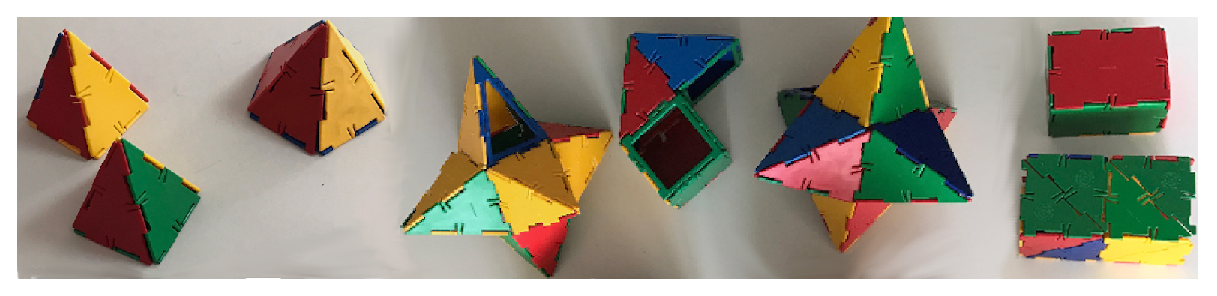
\includegraphics[width=15cm]{polydrons} \\
      \end{center}
   \end{QCM}
\end{activite}


%%%%%%%%%%%%%%%%%%%%%%%%%%%%%%%%%%%%
\cours 

%%%%%%%%%%%%%%%%%%%%%%%%%%%%%%%%
\section{Vocabulaire des solides}

{\psset{yunit=0.95}
\begin{pspicture}(0,0)(17,21)
   \psline[linestyle=dotted](0,10)(5.8,10)
   \psline[linestyle=dotted](12.8,10)(17,10)
   \rput(9.25,10){\ovalnode{A}{\Large Les solides du collège}}
   \rput{90}(0,5){\textcolor{B2}{\large Les solides non polyédriques}}
   \rput{90}(0,15){\textcolor{A1}{\large Les polyèdres}}
   %prisme
   \psnode(6,12.5){B}{\begin{minipage}{10.5cm}{\bf Prisme} : du grec {\it prismatos}, scié. Deux bases polygonales, des faces latérales qui sont des parallélogrammes, rectangles si le prisme est droit.\end{minipage}}
   \rput(5,13.5){{\psset{unit=0.35}\psSolid[object=prisme,h=0.8,action=draw*,linecolor=A1]}}
   \rput(8.5,14){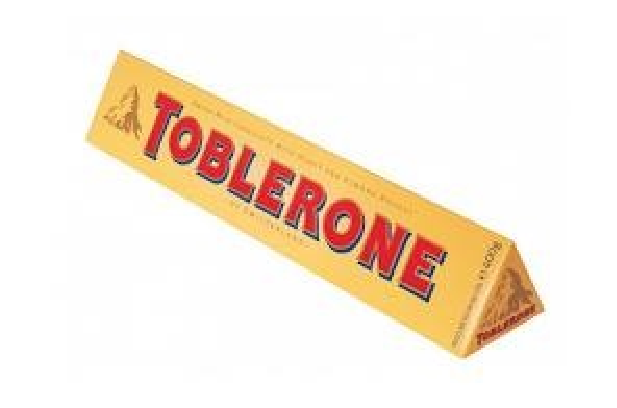
\includegraphics[width=3.25cm]{Cours_Toblerone}}
   \ncline{A}{B}
   \ncput*{\textcolor{A1}{prismes}}
   %pavé 
   \psnode(6,16){D}{\begin{minipage}{10.5cm}{\bf Parallélépipède ou pavé} : du grec {\it parallelos}, parallèle et {\it epidon}, surface. Cas particulier du prisme droit lorsque la base est un rectangle.\end{minipage}}
   \rput(4.5,17.5){\psSolid[object=parallelepiped,a=0.6,b=0.4,c=0.3,action=draw*,linecolor=A1]}
   \rput(8.5,17.5){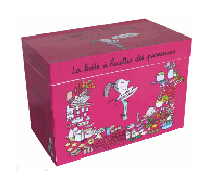
\includegraphics[width=2.5cm]{Cours_boite}}
   \psnode(6,13){G}{} 
   %\ncline{G}{D}
   %cube
   \psnode(6,19.5){E}{\begin{minipage}{10.5cm}{\bf Cube} : cas particulier du pavé droit lorsque toutes les faces sont carrées.\end{minipage}}
   \rput(4.5,21){\psSolid[object=parallelepiped,a=0.5,action=draw*,RotX=30,linecolor=A1]}
   \rput(8.5,21){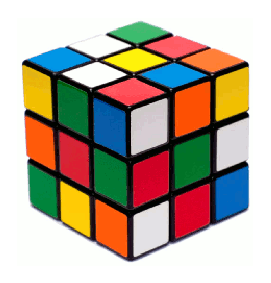
\includegraphics[width=2cm]{Cours_Rubiks}}
   \psnode(6,17){F}{}
   %\ncline{F}{E}
   %Pyramide
   \psnode(14.75,14){C}{\begin{minipage}{4.5cm}{\bf Pyramide} : une base polygonale, un sommet, des faces latérales triangulaires, qui sont isocèles et superposables si la pyramide est régulière.\end{minipage}}
   \rput(15,17){\psSolid[object=tetrahedron,r=0.6,action=draw*,RotZ=70,linecolor=A1]}
   \rput(14.75,20.5){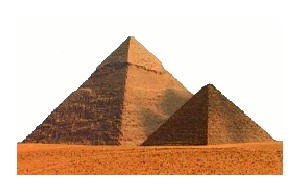
\includegraphics[width=4.5cm]{Cours_Kheops}}
   \ncline{A}{C}
   \ncput*{\textcolor{A1}{pyramides}}
   %Cylindre
   \psnode(3.75,6.5){D}{\begin{minipage}{4.5cm}{\bf Cylindre} : du grec {\it kulindros}, rouleau. Deux bases en forme de disques, une surface latérale.\end{minipage}}
   \rput(4.5,3.5){\psSolid[object=cylindre,h=1,r=0.2,action=draw**,
ngrid=8 16,RotX=90,linecolor=B2]}
   \rput(3.75,1){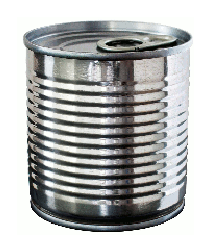
\includegraphics[height=2.75cm]{Cours_conserve}}
   \ncline{A}{D}
   \ncput*{\textcolor{B2}{cylindres}}
   %Cône
   \psnode(9.25,6.5){D}{\begin{minipage}{4.5cm}{\bf Cône} : du grec {\it kônos}, pomme de pin. Une base en forme de disque, une surface latérale, un sommet. \end{minipage}}
   \rput(9.25,4.85){\psSolid[object=cone,h=0.8,r=0.4,action=draw**,ngrid=8 16,RotX=200,linecolor=B2]
}
   \rput(10,1){
\includegraphics[height=3cm]{Cours_glace}}
   \ncline{A}{D}
   \ncput*{\textcolor{B2}{cônes}}
   %Sphère
   \psnode(14.75,6.5){D}{\begin{minipage}{4.5cm}{\bf Sphère} : du grec {\it sphaîra}, corps rond, est la surface extérieure de la {\bf boule}. \end{minipage}}
   \rput(14.75,4.15){\psSolid[object=sphere,r=0.45,ngrid=18 18,linecolor=B2]}
   \rput(14.75,1){
\includegraphics[height=2.75cm]{Cours_ballon}}
   \ncline{A}{D}
   \ncput*{\textcolor{B2}{boules}}
\end{pspicture}}


%%%%%%%%%%%%%%%%%%%%%%%%
\section{Représenter et construire des solides}

\subsection{Perspective cavalière}

\begin{definition}
   Un \textbf{polyèdre} est un solide de l'espace délimité par un nombre fini de polygones, appelés les faces du polyèdre.
\end{definition}

\bigskip

Pour représenter un solide de l'espace, on utilise généralement la {\bf perspective cavalière} : technique de dessin permettant de représenter un solide sur une surface à deux dimensions en respectant le parallélisme.

\begin{exemple}
   Représentation d'un parallélépipède rectangle en perspective cavalière :
   \begin{enumerate}
      \item on trace en vraie grandeur la face de devant ;
      \item on trace les arêtes visibles des faces latérales parallèles et de même longueur : ce sont les fuyantes, plus courtes que leur mesure réelle ;
      \item on trace les arêtes visibles de la face arrière ;
      \item on trace les arêtes cachées en pointillés.
   \end{enumerate}
   \correction
      {\psset{unit=0.9}
      \begin{pspicture}(-3,-0.5)(5,3)
         \pspolygon(0,0)(4,0)(5,1)(5,3)(1,3)(0,2)
         \psline(0,2)(4,2)(4,0)
         \psline(4,2)(5,3)
         \psline[linestyle=dashed](0,0)(1,1)(5,1)
         \psline[linestyle=dashed](1,1)(1,3)
         \rput(0,-0.3){A}
         \rput(4,-0.3){B}
         \rput(5.1,0.7){C}
         \rput(1.2,0.7){D}
         \rput(0,2.3){E}
         \rput(4,2.3){F}
         \rput(5,3.3){G}
         \rput(1,3.3){H}
      \end{pspicture}} \\
      Ce parallélépipède rectangle possède :
      \begin{itemize}
         \item $8$ \textbf{sommets} : $A$, $B$, $C$, $D$, $E$, $F$, $G$ et $H$ ;
         \item $12$ \textbf{arêtes} : $[AB]$, $[BC]$, $[AE]$, $[BF]$, $[EF]$, $[FG]$, $[CG]$, $[EH]$ et $[GH]$ apparentes, et $[AD]$, $[DC]$ et $[DH]$ cachées ;
         \item 6 \textbf{faces} : $ABFE$ est la face de devant, $CDHG$ celle de derrière, $ABCD$ la face du dessous, $EFGH$ celle du dessus, $BCGF$ la face de droite, et $ADHE$ celle de gauche.
      \end{itemize}
\end{exemple}


%%%%%%%%%%%%%%%%%%%%%%%%%
\subsection{Patron}

\begin{definition}
   Le \textbf{patron} d'un solide est une surface plane d'un seul tenant qui, par pliage, permet de reconstituer le solide sans recouvrement de ses faces.
\end{definition}

\bigskip

On \og déplie \fg{} le parallélépipède rectangle pour en obtenir un de ses patrons :

\begin{exemple}
   \qquad 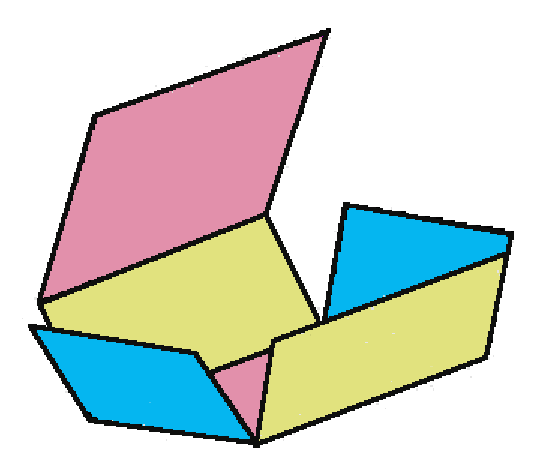
\includegraphics[width=4.9cm]{Cours_pave_deplie}\correction
{\psset{unit=0.9}
\begin{pspicture}(-2,-0.5)(6,4.5)
   \psline(1,0)(1,1)(0,1)(0,3.5)(1,3.5)(1,4.5)(3,4.5)(3,3.5)(4,3.5)(6,3.5)(6,1)(4,1)(3,1)(3,0)(1,0)
   \psframe(1,1)(3,3.5)
   \psline(4,3.5)(4,1)
   \rput(0.5,1){\textcolor{B2}{x}}
   \rput(1,0.5){\textcolor{B2}{x}}
   \rput(0.5,3.5){\textcolor{B2}{x}}
   \rput(1,4){\textcolor{B2}{x}}
   \rput(3.5,1){\textcolor{B2}{x}}
   \rput(3,0.5){\textcolor{B2}{x}}
   \rput(3.5,3.5){\textcolor{B2}{x}}
   \rput(3,4){\textcolor{B2}{x}}
   \rput(0,2.25){\textcolor{A1}{o}}
   \rput(1,2.25){\textcolor{A1}{o}}
   \rput(3,2.25){\textcolor{A1}{o}}
   \rput(4,2.25){\textcolor{A1}{o}}
   \rput(6,2.25){\textcolor{A1}{o}}
   \rput(2,0){\textcolor{J1}{|\!\!|}}
   \rput(2,1){\textcolor{J1}{|\!\!|}}
   \rput(2,3.5){\textcolor{J1}{|\!\!|}}
   \rput(2,4.5){\textcolor{J1}{|\!\!|}}
   \rput(5,1){\textcolor{J1}{|\!\!|}}
   \rput(5,3.5){\textcolor{J1}{|\!\!|}}
\end{pspicture}}
\end{exemple}

\bigskip

Le patron d'un polyèdre n'est pas unique, il dépend de la manière dont on le déplie. \\
 On ne parle de patron que pour un polyèdre. On parle de développement pour un cylindre ou un cône.


%%%%%%%%%%%%%%%%%%%%%%%%%%%%%%%%%%%%%%%%%%
\exercicesbase

\begin{colonne*exercice}

\serie{Classer et reconnaître des solides} %%%

\begin{exercice} %1
   On considère les catégories de solides suivants que l'on peut trouver dans la vie courante :
   \begin{enumerate}
      \item[A.] Différentes boites parallélépipédiques et cubiques.
      \item[B.] Des prismes droits à bases triangulaires (Toblerone) ou octogonales.
      \item[C.] Une pyramide à base carrée tronquée (boite de fromage de chèvre).
      \item[D.] Des cylindres (boîtes de conserve diverses, boîte de camembert, rouleau de papier d'aluminium).
      \item[E.] Des cônes.
      \item[F.] Des boules (balles, ballons).
      \item[G.] D'autres emballages (formes ovales, anneaux, boîtes en forme de c\oe ur\dots).
   \end{enumerate}
   \vspace*{-5mm}
   \begin{enumerate}
      \item Classer ces sept catégories selon leur caractère polyédrique ou non
      \item Pourquoi, en cours de maths, faut-il s'intéresser uniquement aux formes des boites d'emballages ?
      \item Quelle est la particularité du rouleau de papier d'aluminium ?
      \item Des classes ont proposé les classements suivants : \smallskip
      \begin{center}
         \hautab{1}
         \begin{ltableau}{0.55\linewidth}{2}
            \hline
            5\up{e}1 & 5\up{e}2 \\
            \hline
            A, B et C & A, B et D \\
            F & C et E \\
            G & F et G \\
            \hline
         \end{ltableau}
      \end{center}
      \medskip
      Quels ont pu être leurs critères de classement ?
      \item On propose la définition suivante pour déterminer un polyèdre : \og solide qui ne roule pas \fg{} et pour un non polyèdre : \og solide qui roule \fg. \\
      Ces définitions vous paraissent-elles pertinentes ?
   \end{enumerate}
\end{exercice}

\begin{exercice} %2
   On dispose de trois objets sur une table : un cône, un cube et une sphère. On a également des représentations de ces solides selon des points de vue différents : \\
   Vue de la table du dessus : 
   \begin{center}
      \begin{pspicture}(-2.3,-2.3)(2.3,2.3)
         \psframe(-1.5,-1.5)(1.5,1.5)
         \rput(2,2){NE}
         \rput(1.7,1.7){$\swarrow$}
         \rput(2,0){E}
         \rput(1.7,0){$\leftarrow$}
         \rput(2,-2){SE}
         \rput(1.7,-1.7){$\nwarrow$}
         \rput(0,-2){S}
         \rput(0,-1.7){$\uparrow$}
         \rput(-2,-2){SO}
         \rput(-1.7,-1.7){$\nearrow$}
         \rput(-2,0){O}
         \rput(-1.7,0){$\rightarrow$}
         \rput(-2,2){NO}
         \rput(-1.7,1.7){$\searrow$}
         \rput(0,2){N}
         \rput(0,1.7){$\downarrow$}
         \pscircle(0.6,-0.85){0.45}
         \pscircle(-0.25,0.85){0.45}
         \pscircle(-0.25,0.85){0.05}
         \pspolygon(-1,-0.4)(-0.55,0.35)(0.2,-0.1)(-0.25,-0.85)
      \end{pspicture}
   \end{center}
   Solides en vue du dessus et de face :
   \begin{center}
      \begin{pspicture}(0,-1.5)(8,1.7)
          \rput[l](0.5,1){vue aérienne}
          \pscircle(3.5,1){0.45}
          \pscircle(3.5,1){0.05}
          \pscircle(5.25,1){0.45}
          \rput(7.4,1.25){\pspolygon(-1,-0.4)(-0.55,0.35)(0.2,-0.1)(-0.25,-0.85)}
          \rput[l](0.5,-0.5){vue frontale}
          \rput(3.05,-1.3){\cone}
          \rput(5.25,-.95){\boule}
          \rput(6.4,-0.95){\cube}
      \end{pspicture}
   \end{center} 
   Les images ci-dessous représentent des vues, selon divers axes de visée. Déterminer le point de vue de chaque image (attention, certaines images ne correspondent à aucune configuration !). \\ [2mm]
   {\hautab{1.5}
   \begin{ltableau}{\linewidth}{8}
      \hline
      N & NE & E & SE & S & SO & O & NO \\
      \hline
      & & & & & & & \\
      \hline
   \end{ltableau}}
\end{exercice}      
\end{colonne*exercice}

\begin{center}
   \begin{pspicture}(0,0)(3.3,2.9)
      \psframe(0,0)(3.2,2.5)
      \rput(2.9,2.2){A}
      \rput(0.9,0.2){\boule}
      \rput(1.35,0.2){\cube}
      \rput(1.35,0.2){\cone}
   \end{pspicture}
   \begin{pspicture}(0,0)(3.3,2.9)
      \psframe(0,0)(3.2,2.5)
      \rput(2.9,2.2){B}
      \rput(0.2,0.2){\cone}
      \rput(2.3,0.2){\boule}
      \rput(1.1,0.2){\cube} 
   \end{pspicture}
   \begin{pspicture}(0,0)(3.3,2.9)
      \psframe(0,0)(3.2,2.5)
      \rput(2.9,2.2){C}
      \rput(2.15,0.2){\boule}
      \rput(0.8,0.2){\cone}
      \rput(0.55,0.2){\cube}      
   \end{pspicture}
   \begin{pspicture}(0,0)(3.3,2.9)
      \psframe(0,0)(3.2,2.5)
      \rput(2.9,2.2){D}
      \rput(1.4,0.2){\cube}  
      \rput(0.4,0.2){\cone}
      \rput(0.85,0.2){\boule}
   \end{pspicture}
   \begin{pspicture}(0,0)(3.3,2.9)
      \psframe(0,0)(3.2,2.5)
      \rput(2.9,2.2){E}
      \rput(0.65,0.2){\cube}
      \rput(0.75,0.2){\boule}
      \rput(1.9,0.2){\cone}
   \end{pspicture} \\
   \begin{pspicture}(0,0)(3.3,2.7)
      \psframe(0,0)(3.2,2.5)
      \rput(2.9,2.2){F}
      \rput(1.6,0.2){\boule}
      \rput(1.3,0.2){\cubeg}
      \rput(0.5,0.2){\cone}
   \end{pspicture}
   \begin{pspicture}(0,0)(3.3,2.7)
      \psframe(0,0)(3.2,2.5)
      \rput(2.9,2.2){G}
      \rput(0.3,0.2){\cone}
      \rput(2.55,0.2){\boule}
      \rput(0.8,0.2){\cubeg} 
   \end{pspicture}
   \begin{pspicture}(0,0)(3.3,2.7)
      \psframe(0,0)(3.2,2.5)
      \rput(2.9,2.2){H}
      \rput(0.6,0.2){\cone}
      \rput(1.4,0.2){\cubeg}
      \rput(1.6,0.2){\boule}   
   \end{pspicture}
   \begin{pspicture}(0,0)(3.3,2.7)
      \psframe(0,0)(3.2,2.5)
      \rput(2.9,2.2){I}
      \rput(1.6,0.2){\cone}
      \rput(0.6,0.2){\cubeg}  
      \rput(1.5,0.2){\boule}
   \end{pspicture}
   \begin{pspicture}(0,0)(3.3,2.7)
      \psframe(0,0)(3.2,2.5)
      \rput(2.9,2.2){J}
      \rput(1.2,0.2){\cubeg}
      \rput(0.65,0.2){\boule}
      \rput(2,0.2){\cone}
   \end{pspicture}
\end{center}
   

\serie{Représenter et construire des solides} %%%

\begin{exercice}
   Terminer la représentation en perspective cavalière des trois pavés suivants :
   \begin{center}
  {\psset{unit=0.65}
      \begin{pspicture}(-1,-1)(22,6)
      \psgrid[subgriddiv=1,gridlabels=0pt,gridcolor=gray](-1,-1)(22,6)
      \psset{linewidth=0.7mm}
      \psline(0,2)(0,0)(2,0)(2,2)(3,3)% cube
      \psline[linestyle=dashed](0,0)(1,1)
      \psline(8,0)(5,0)(5,4)(8,4)(10,5)%pavé
      \psline[linestyle=dashed](5,0)(7,1)(10,1) 
      \psline[linestyle=dashed](12,0)(13,2)(21,2) % pavé plat
      \psline[linestyle=dashed](13,2)(13,4)
      \psline(12,0)(20,0)(20,2)
   \end{pspicture}}
   \end{center}
\end{exercice}

\begin{exercice} %2
   Tracer un maximum de patrons différents du cube (c'est-à-dire non superposables).
\end{exercice}

\begin{exercice}
   On donne le patron d'un dé, compléter les autres patrons du même dé. \\
   \begin{pspicture}(0,0)(17,4.3)
   \psset{unit=0.9}
      \def\car{\psframe(0,0)(1,1)}
      \rput(0,3){\car} \rput(1,3){\car} \rput(1,2){\car} \rput(1,1){\car} \rput(2,1){\car} \rput(2,0){\car}
      \rput{90}(0.5,3.5){\psdice{3}} \rput(1.5,3.5){\psdice{2}} \rput(1.5,2.5){\psdice{6}} \rput(1.5,1.5){\psdice{5}} \rput(2.5,1.5){\psdice{4}} \rput(2.5,0.5){\psdice{1}} %1
      \rput(4,3){\car} \rput(5,3){\car} \rput(5,2){\car} \rput(6,2){\car} \rput(6,1){\car} \rput(7,1){\car}
      \rput{90}(4.5,3.5){\psdice{3}} \rput(5.5,2.5){\psdice{1}}
      %2
      \rput(9,3){\car} \rput(10,3){\car} \rput(10,2){\car} \rput(11,2){\car} \rput(12,2){\car} \rput(11,1){\car} %3
      \rput{90}(9.5,3.5){\psdice{6}} \rput(10.5,2.5){\psdice{4}} \rput(11.5,2.5){\psdice{1}}
      \rput(14,0){\car} \rput(15,0){\car} \rput(16,0){\car} \rput(15,1){\car} \rput(15,2){\car} \rput(15,3){\car}
      \rput(15.5,2.5){\psdice{5}} \rput(15.5,1.5){\psdice{1}} \rput(16.5,0.5){\psdice{4}}
      %4
   \end{pspicture}
\end{exercice}

\begin{exercice}
   Construire en vraie grandeur le patron d'un pavé droit de mesures \ucm{5}, \ucm{4} et \ucm{3}. Auparavant, on fera un schéma à main levée.
\end{exercice}

\medskip

\begin{exercice}
Reproduire la figure suivante en perspective isométrique juste à côté : combien y a-t-il de cubes entiers ? Et si on retourne la figure ? \\ [2mm]
{\psset{unit=0.5}

\begin{pspicture*}(-3,5)(30,18)
   %quadrillage
   \multido{\n=0+2}{15}{\psline[linestyle=dotted](\n,-2)(\n,20)}
   \multido{\i=-15+2,\n=0+2}{18}{\psline[linestyle=dotted](-1,\i)(29,\n)}
   \multido{\i=-15+2,\n=0+2}{18}{\psline[linestyle=dotted](-1,\n)(29,\i)} 
   %pyramide
   \cubiso{6}{12.5}
   \cubiso{4}{9.5}
   \cubiso{2}{6.5}
   \cubiso{8}{9.5}
   \cubiso{6}{6.5}
   \cubiso{10}{6.5} 
   \pspolygon[fillstyle=solid,fillcolor=black](2,6.5)(4,5.5)(6,6.5)(4,7.5)
   \pspolygon[fillstyle=solid,fillcolor=black](8,5.5)(10,6.5)(8,7.5)(6,6.5)
   \pspolygon[fillstyle=solid,fillcolor=red](12,9.5)(12,11.5)(10,12.5)(10,10.5)
   \pspolygon[fillstyle=solid,fillcolor=red](10,12.5)(10,14.5)(8,15.5)(8,13.5)
   \pspolygon[fillstyle=solid,fillcolor=lightgray](0,9.5)(2,10.5)(2,12.5)(0,11.5)
   \pspolygon[fillstyle=solid,fillcolor=lightgray](2,12.5)(4,13.5)(4,15.5)(2,14.5)    
\end{pspicture*}}
\end{exercice}


%%%%%%%%%%%%%%%%%%%%%%%%%%%%%%%%%%%%%%%%%%
%%%%%%%%%%%%%%%%%%%%%%%%%%%%%%%%%%%%%%%%%%
\Recreation

\enigme[La relation d'Euler\footnote{Leonhard Euler, né le 15 avril 1707 à Bâle (Suisse) et mort à 76 ans le 7 septembre 1783 à Saint-Pétersbourg (Empire russe), est un mathématicien et physicien suisse.}]
   On a reproduit page suivante une représentation en perspective cavalière de neuf solides. Pour chacun de ces solides, effectuer les actions suivantes à l'aide du tableau ci-dessous :
   \begin{itemize}
      \item retrouver son nom dans le tableau (indiquer le numéro n) ;
      \item trouver le nombre de faces F ;
      \item trouver le nombre de sommets S ;
      \item trouver le nombre d'arêtes A ;
      \item calculer la valeur de F + S $-$ A, que remarque-t-on ?
      \item dire si le solide est régulier, c'est-à-dire si toutes ses faces sont identiques et régulières, et tous les angles du solide sont identiques ;
      \item dire si le solide est convexe, c'est à dire s'il n'a pas de \og creux \fg{} ou de trou ;
      \item enfin, dire s'il s'agit d'un solide de Platon (polyèdre régulier et convexe).
   \end{itemize}
   \begin{center}   
      {\hautab{2.2}
      \begin{CLtableau}{0.958\linewidth}{9}{C{3}|C{0.9}|C{0.9}|C{0.9}|C{0.9}|C{1.4}|C{1.4}|C{1.4}|C{1.4}}
         \hline
         Nom du solide & n & F & S & A & F + S $-$ A & est-il régulier ? & est-il convexe ? & solide de Platon ?\\
         \hline
         Tétraèdre & & & & & & & & \\
         \hline
         Polyèdre étoilé & & & & & & & & \\
         \hline
         Octaèdre & & & & & & & & \\
         \hline
         Pyramide & & & & & & & & \\
         \hline
          Icosaèdre & & & & & & & & \\
         \hline
         Prisme & & & & & & & & \\
         \hline
          Cube & & & & & & & & \\
         \hline
         Beignoïde  & & & & & & & & \\
         \hline
         Dodécaèdre & & & & & & & & \\
         \hline    
   \end{CLtableau} }
   \end{center}
   \hfill{\footnotesize\it Source : d'après une activité parue dans la revue {\it Envol}. n\degre129, octobre-novembre-décembre 2004.}
   
\pagebreak

   {\psset{unit=0.9}
   \begin{pspicture}(-4,-6)(18,18)
      \rput(12,16){\psSolid[object=cube,a=1,RotZ=20,action=draw*, fillcolor=orange!20] \\
         {\Huge2}}
      \rput(6,-4){\psSolid[object=tetrahedron,r=1.1,RotZ=20,action=draw*,fillcolor=A1!20] \\
          {\Huge9}}
      \rput(12,0){\psSolid[object=dodecahedron,a=0.9,RotZ=0,action=draw*,fillcolor=B2!20] \\
          {\Huge8}}
      \rput(0,8){\psSolid[object=octahedron,a=1,RotZ=20,action=draw*,fillcolor=yellow!20] \\
          {\Huge4}}
      \rput(6,4){\psSolid[object=icosahedron,a=1,RotZ=60,action=draw*,fillcolor=lightgray!20] \\
          {\Huge6}}
      \rput(12,7.7){\psSolid[object=prisme,h=0.6,RotZ=10,action=draw*,fillcolor=green!20] \\
          {\Huge5}}
      \rput(0,17){\psSolid[object=new, sommets=0 -0.7 0 -0.7 0 0 0 1 0 1 0 0 0 0 -2,faces={[3 2 1 0][4 0 3][4 3 2][4 2 1][4 1 0]},RotZ=40,action=draw*,fillcolor=magenta!20]{\Huge 1}}
      \rput(5.5,12){\psSolid[object=anneau,r=0.4,R=1,h=1.5,ngrid=4,RotZ=30,RotY=50,action=draw*,fillcolor=cyan!20] \\
         {\Huge 3}}
      \rput(0,0){\psSolid[object=new,sommets=-0.3 -0.3 -0.3 0.3 -0.3 -0.3 0.3 0.3 -0.3 -0.3 0.3 -0.3 -0.3 -0.3 0.3 0.3 -0.3 0.3 0.3 0.3 0.3 -0.3 0.3 0.3 1.5 0 0 0 1.5 0 0 0 1.5 0 0 -1.5 -1.5 0 0 0 -1.5 0,faces={[1 2 6 5][0 3 2 1][4 5 6 7][0 1 5 4][3 7 6 2][0 4 7 3][11 3 2][11 0 3][11 1 0][11 2 1][12 7 3][12 4 7][12 0 4][12 3 0][13 1 5][13 0 1][13 4 0][13 5 4][8 2 6][8 6 5][8 5 1][8 1 2][9 3 7][9 7 6][9 6 2][9 2 3][10 6 7][10 5 6][10 7 4][10 4 5]},RotZ=20,RotX=10,action=draw*,fillcolor=green!20] \\
         {\Huge7}}
   \end{pspicture}} 
 